\section{Durchführung}
\label{sec:Durchführung}

\subsection{Aufbau und Funktionsweise}
\begin{figure}[H]
    \centering
        \centering
        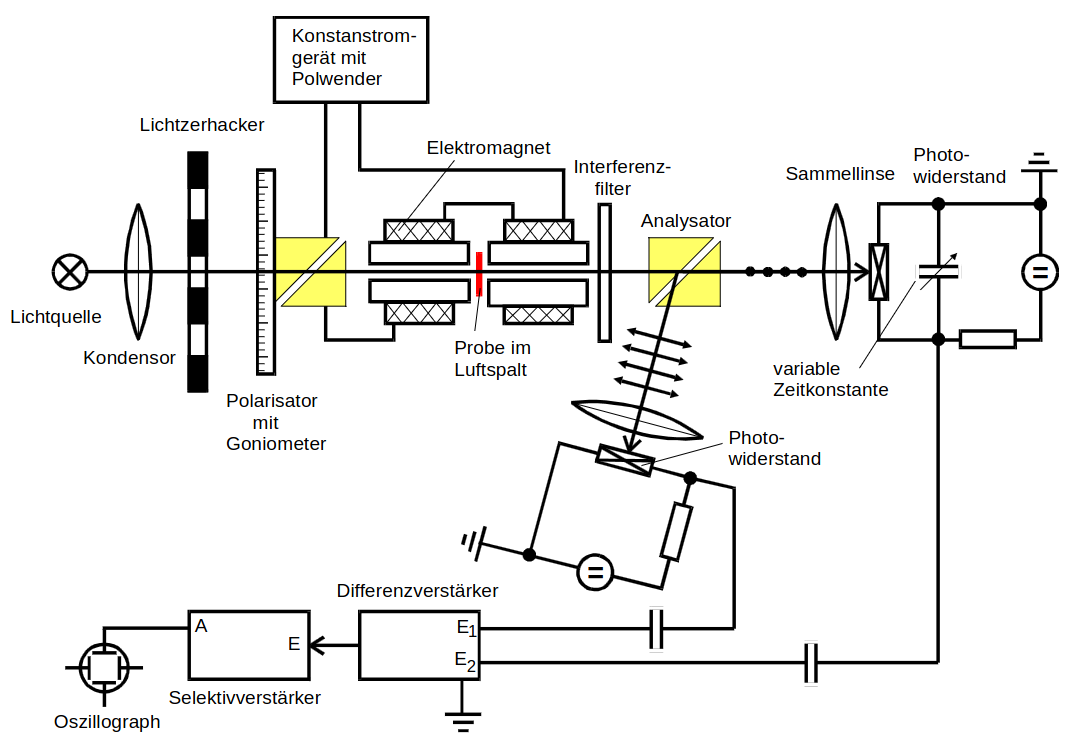
\includegraphics[width=0.65\textwidth]{Bilder/schemaAufbau.png}
        \caption{Schematische Aufbau der Apperatur. \cite{v46anhang}}
    \hfill
    \label{fig:4}
\end{figure}
\noindent In \autoref{fig:4} ist eine Skizze der Messutensilien dargestellt.
Angefangen links, befindet sich die Lichtquelle. Dabei handelt es sich um eine 
Halogen-Lampe, welche infrarotes Licht emittiert. Diese Lichtquelle wird gewählt, 
da die Proben infrarot-durchlässig sind. Dahinter befindet sich der Kondensor, 
welcher das Licht der Quelle in parallele Strahlen umwandelt. Das hat den Zweck, 
das eintreffende Licht zu entbündeln, so treffen im späteren Verlauf alle 
Lichtstrahlen unter dem gleichen Winkel auf die Probe. Dahinter liegt der 
Lichtzerhacker, welcher das Licht moduliert. Er besteht aus einer Scheibe mit vielen 
Schlitzen, sodass er nach Einschalten das Licht mit einer Frequenz von $\qty{450}{\hertz}$
periodisch unterbricht. Diese Modulation ist notwendig, damit der Lock-in-Verstärker
im späteren Verlauf das Rauschen von der Umgebung rausfiltern kann. Es folgt das 
erste Glan-Thompson-Prisma, ein anisotropes Medium, welches das Licht in zwei senkrecht 
zueinander polarisierte Strahlen aufteilt (siehe \autoref{fig:5}). Für das Experiment
wird nur der ordentliche Strahl genutzt, welcher das Prisma ungehindert durchläuft. 
\begin{figure}[H]
    \centering
        \centering
        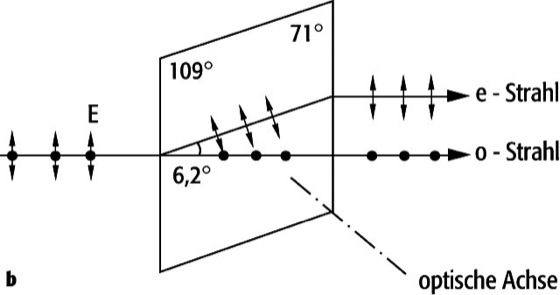
\includegraphics[width=0.65\textwidth]{Bilder/e_o_strahlen.jpg}
        \caption{Doppelbrechung am Glan-Thompson-Prisma mit ordentlichem und außerordentlichem Strahl. \cite{glanthompson}}
    \hfill
    \label{fig:5}
\end{figure}
\noindent Dieses dient als Polarisator, zur Feinjustage wird das angebrachte 
Goniometer genutzt. Es folgt die Probe, welche in einem Elektromagneten liegt. 
Dieser ist ein Konstantstromgerät inklusive Polwender angeschlossen. Der 
Elektromagnet erzeugt ein Magnetfeld, welches parallel zur Ausbreitungsrichtung des
Lichts liegt. Der Polwender ermöglicht es, die Richtung des Magnetfelds zu wechseln, 
sodass die Messung für ein breiteres Spektrum an Winkeln durchgeführt werden kann. 
Der tatsächliche Winkel aus der Faraday-Rotation kann dann gemäß
\begin{equation}
    \theta_\text{Faraday} = \frac{1}{2} \left( \theta_1 - \theta_2 \right)
\end{equation}
berechnet werden, wobei $\theta_1$ und $\theta_2$ die gemessenen Winkel für die
beiden Magnetfeldrichtungen sind. Hinter der Probe ist der Interferenzfilter zu 
finden, um das Spektrum des Lichts zu limitieren. Das ist notwendig, da 
$\theta \propto \lambda^2$ ist. Für die Berechnung bedarf es monochromatischer 
Strahlung. Dahinter liegt das zweite Glan-Thompson-Prisma, welches als Analysator
dient. Es spaltet wie das erste Prisma das Licht in einen ordentlichen und 
außerordentlichen Strahl auf, welche jeweils auf eine Sammellinse und dann auf 
einen Photowiderstand zur Detektion treffen. Der Photowiderstand wandelt die
Intensität des Lichts in ein elektrisches Signal um, welches dann vom
Lock-in-Verstärker verarbeitet wird. Vorher gehen die beiden Signale durch einen 
Differenzverstärker, welcher die Signale der beiden Photowiderstände subtrahiert 
und gleiche Eingänge mittels Gleichtaktunterdrückung herausfiltert. Schließlich 
kommt der Selektivverstärker bzw. Lock-in-Verstärker. Er ist so eingestellt, dass
er nur Signale mit der gleichen Frequenz wie die Modulation des Lichtzerhackers
verstärkt, wodurch Störgeräusche effektiv herausgefiltert werden. Zum Ablesen
der Ergebnisse ist ein Oszilloskop angeschlossen, welches die Ausgangssignale des
Lock-in-Verstärkers anzeigt. Bilder der Aufbauten sind in \autoref{fig:6} und
\autoref{fig:7} zu sehen.
\begin{figure}[H]
    \centering
        \centering
        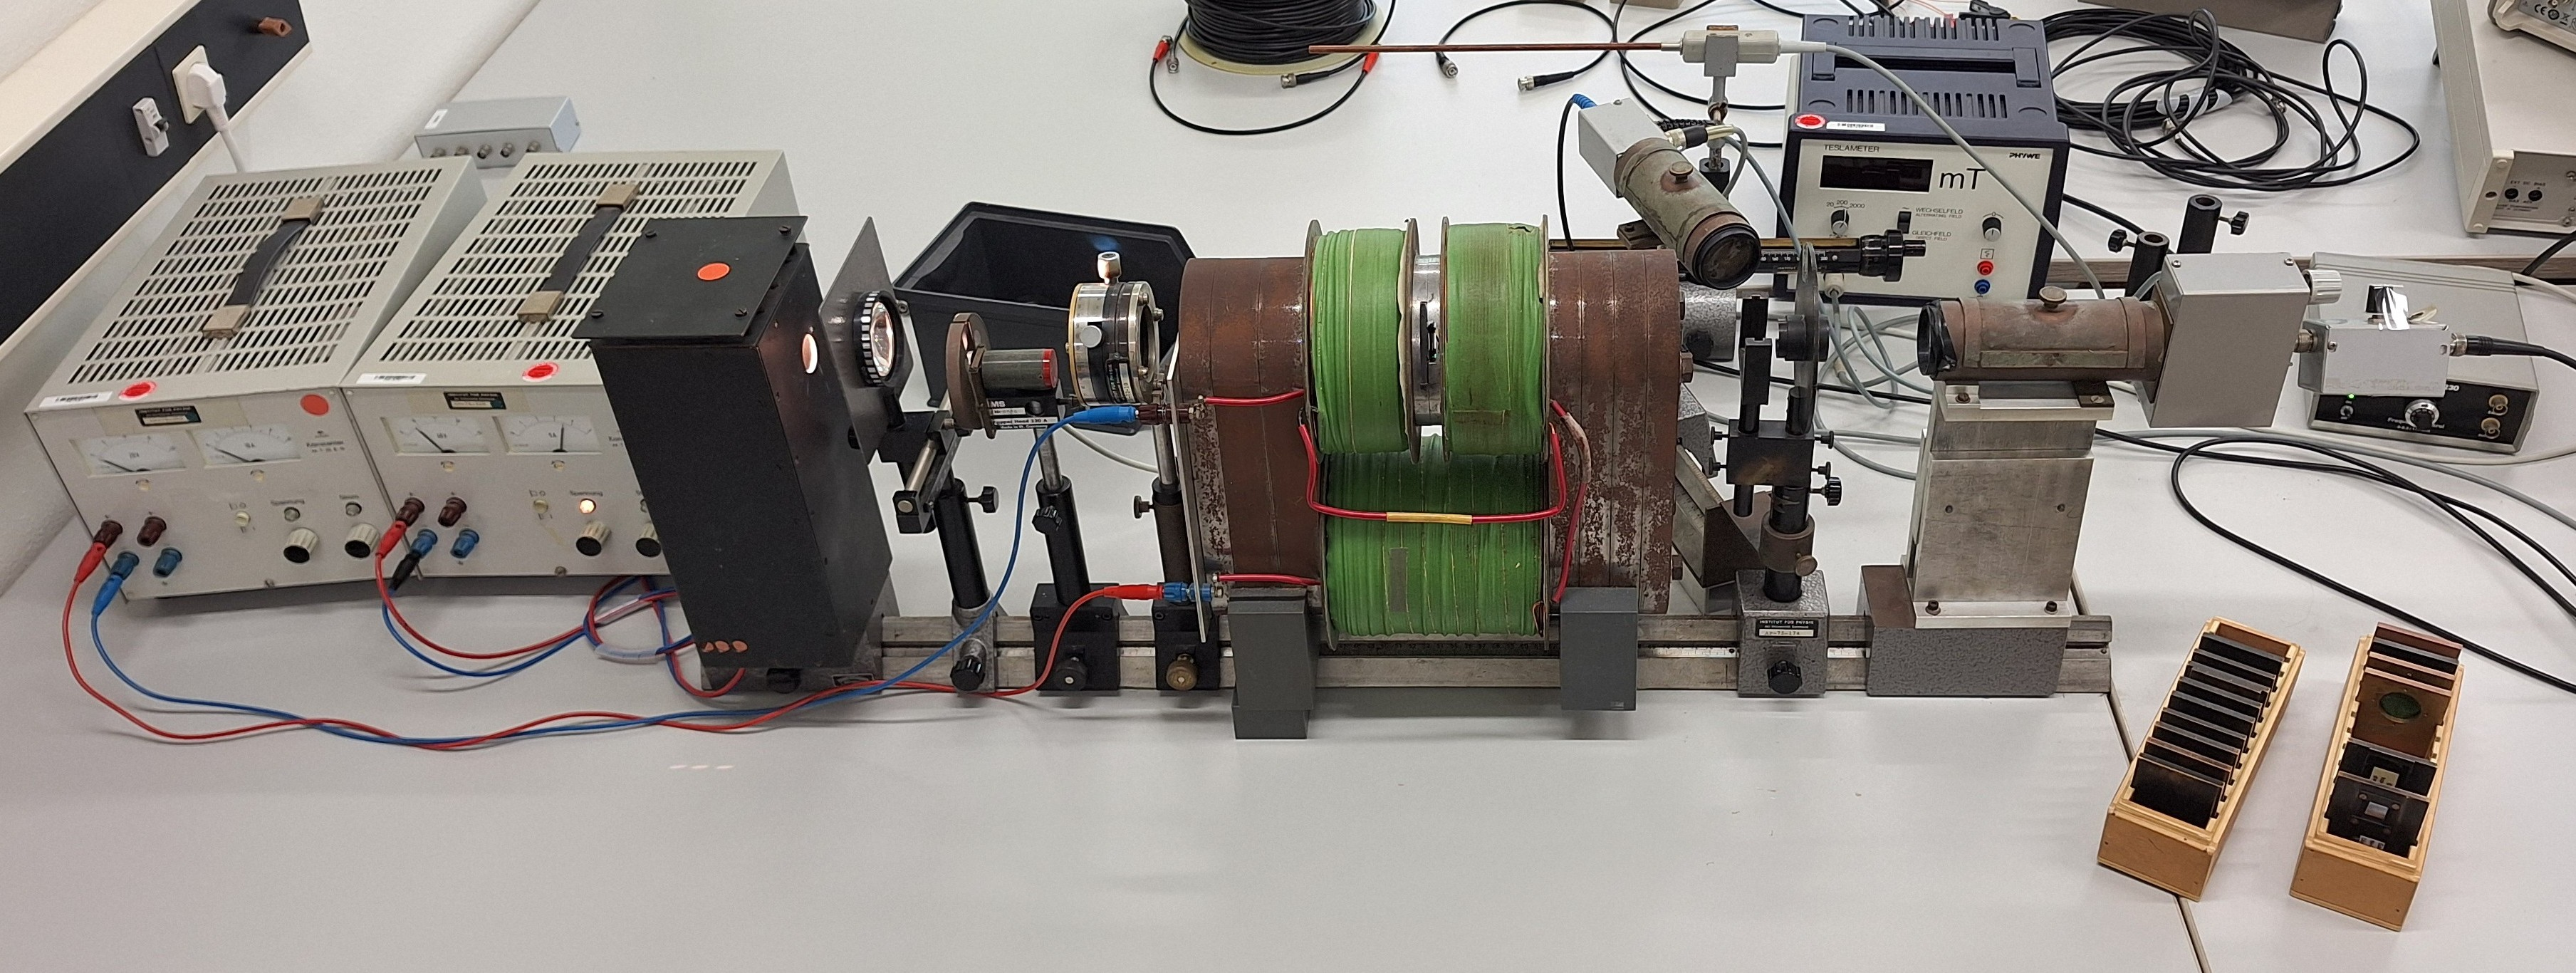
\includegraphics[width=0.85\textwidth]{Bilder/a1.jpg}
        \caption{Aufnahme des Aufbaus von Spannungs-und Lichtquelle (links) bis 
        zu den Photodetektoren (rechts). (Eigenaufnahme)}
    \hfill
    \label{fig:6}
\end{figure}
\begin{figure}[H]
    \centering
        \centering
        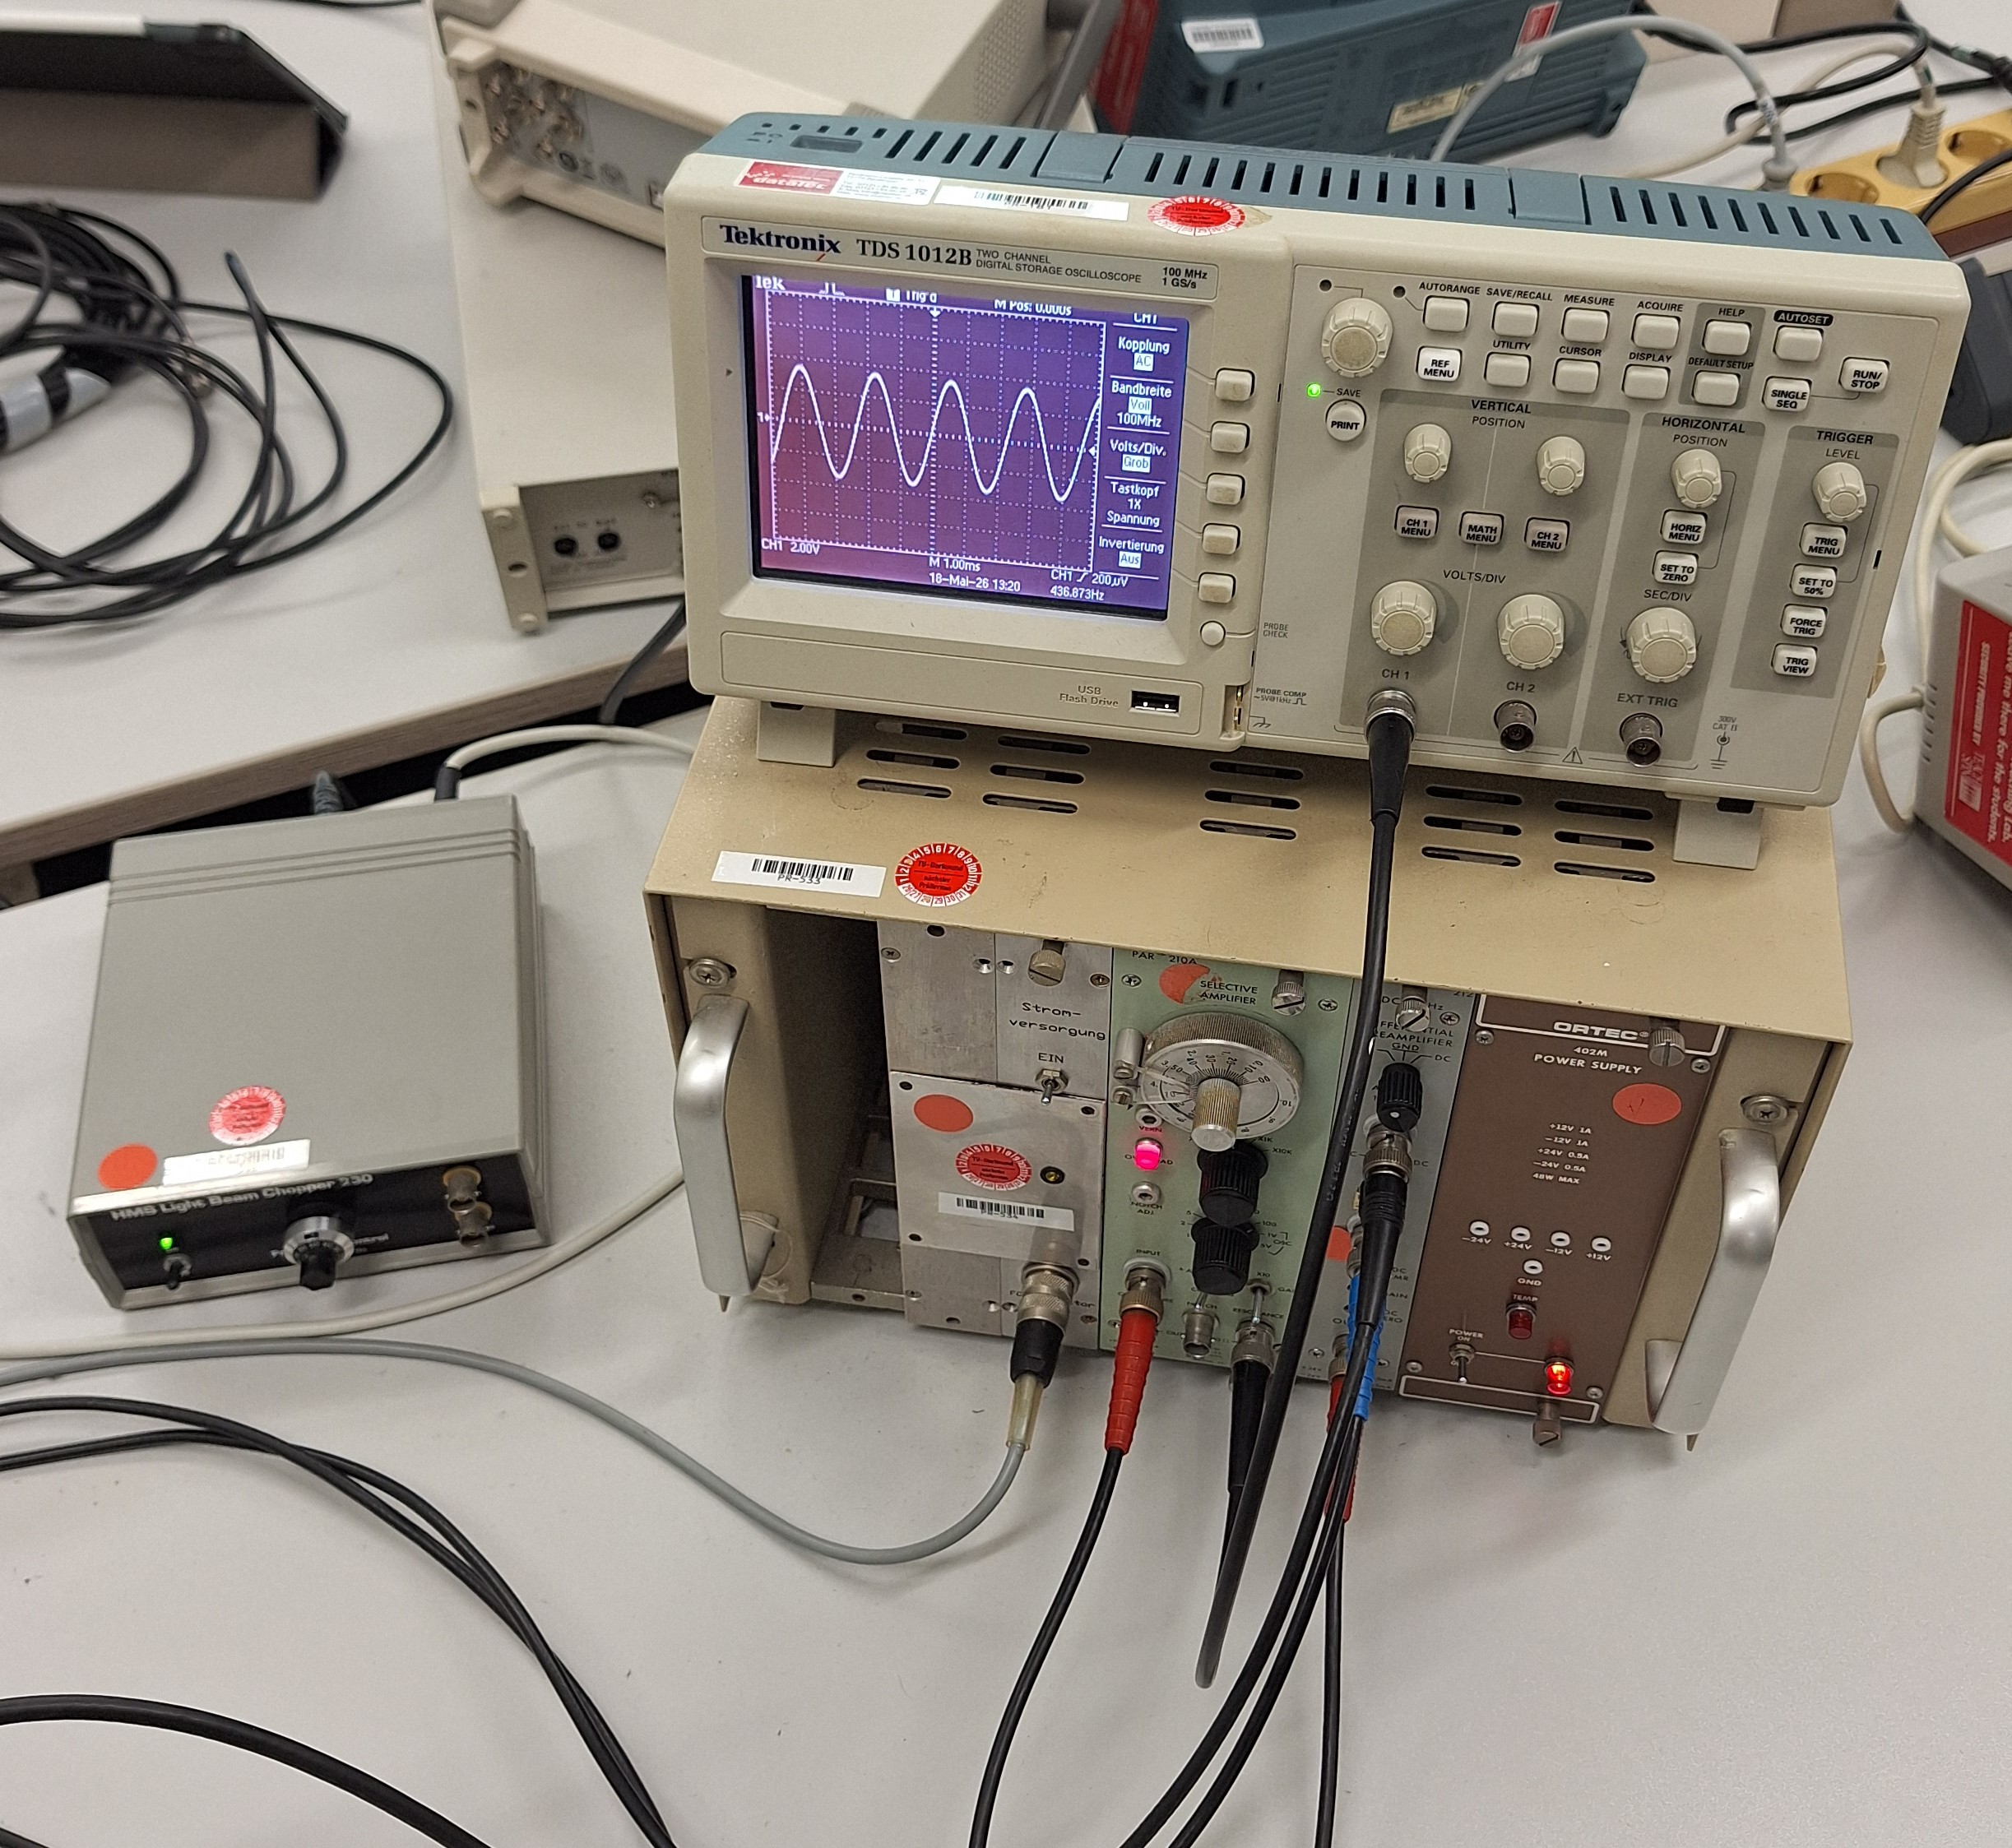
\includegraphics[width=0.55\textwidth]{Bilder/oszillograph.jpg}
        \caption{Aufnahme des Oszillographen. (Eigenaufnahme)}
    \hfill
    \label{fig:7}
\end{figure}


\subsection{Messvorgänge}
\begin{itemize}
    \item Zunächst wird die Nullstellung der Apparatur eingestellt. Dazu wird die 
    Probe entfernt und die beiden Glan-Thompson-Prismen so eingestellt, dass die 
    Intensität des Lichts am Photowiderstand minimal ist. Das bedeutet, dass die
    Polarisationsachsen der beiden Prismen senkrecht zueinander stehen.
    \item Anschließend wird die Probe eingesetzt und das Magnetfeld auf einen Wert von
    $\qty{0.5}{\tesla}$ eingestellt. Es werden Messungen für beide Magnetfeldrichtungen
    durchgeführt, um die Faraday-Rotation zu bestimmen.
    \item Danach wird das Magnetfeld auf $\qty{1.0}{\tesla}$ erhöht und die Messungen
    werden wiederholt.
    \item Schließlich wird das Magnetfeld auf $\qty{1.5}{\tesla}$ erhöht und die Messungen
    werden erneut durchgeführt.
\end{itemize}